\section{Analysis of Features 5 and 6}

\subsection*{Empirical Results}

To conclude our exploratory analysis, we examine Features 5 and 6. This feature pair is the most topologically complex in the entire dataset and represents a severe departure from standard probabilistic assumptions.

\textbf{Distributions and Overlap:}
Based on the histograms (\texttt{feature\_5\_histogram.png} and \texttt{feature\_6\_histogram.png}), a fundamental asymmetry between the classes emerges. The Fake distribution is unimodal (centered near zero) with wide tails. However, the Genuine distribution is strictly \textbf{bimodal}. It exhibits two distinct peaks with a noticeable "valley" or hollow region in the center where the Fake class peaks. 
Consequently, the classes overlap extensively across almost the entire range of values, but they do so in a highly interleaved, non-linear manner.

\textbf{Statistical Metrics:}
The computed statistics confirm this structural density:
\begin{itemize}
    \item \textbf{Means:} Both classes share nearly identical means centered tightly around zero. For Feature 5, the Fake mean is $0.0280$ and Genuine is $-0.0417$. For Feature 6, the Fake mean is $-0.0058$ and Genuine is $-0.0384$.
    \item \textbf{Variances:} The Genuine class exhibits nearly double the variance of the Fake class on both axes. For Feature 5, Fake variance is $0.6801$ while Genuine is $1.3178$. For Feature 6, Fake variance is $0.7050$ while Genuine is $1.2870$.
\end{itemize}

\begin{figure}[H]
    \centering
    \begin{minipage}{0.48\textwidth}
        \centering
        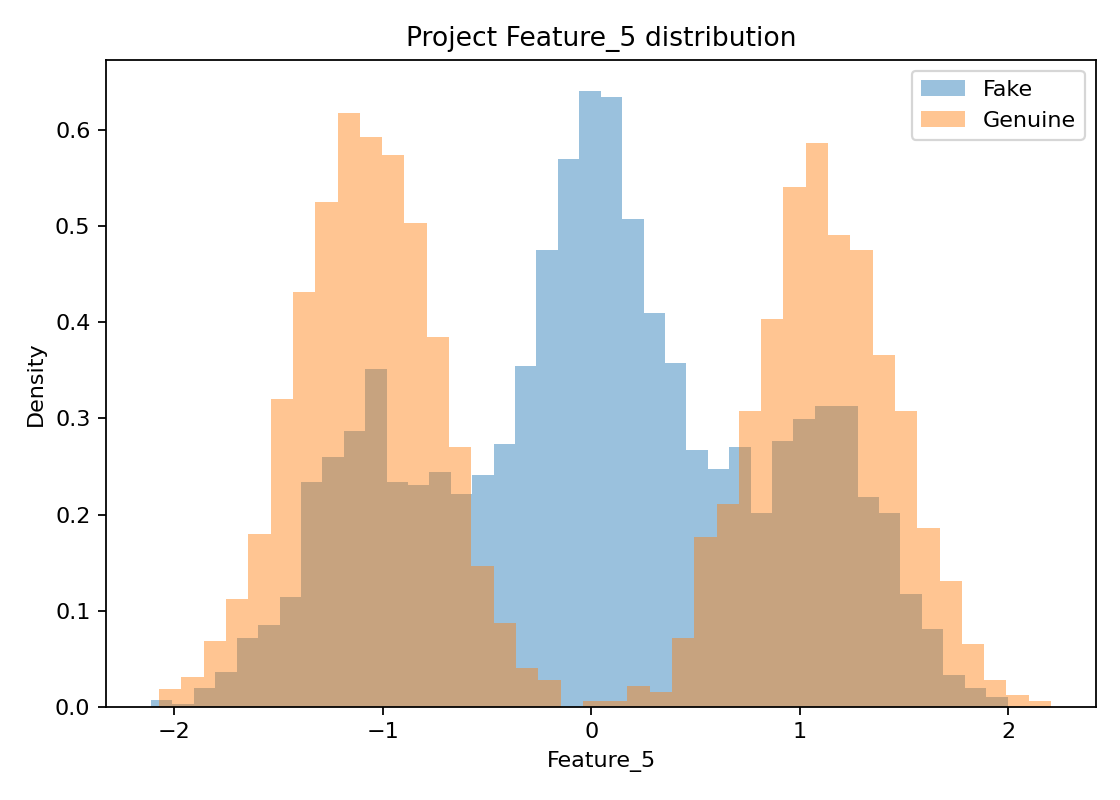
\includegraphics[width=\linewidth]{histograms/feature_5_histogram.png}
        \caption{Histogram of Feature 5, showing Genuine bimodality.}
    \end{minipage}\hfill
    \begin{minipage}{0.48\textwidth}
        \centering
        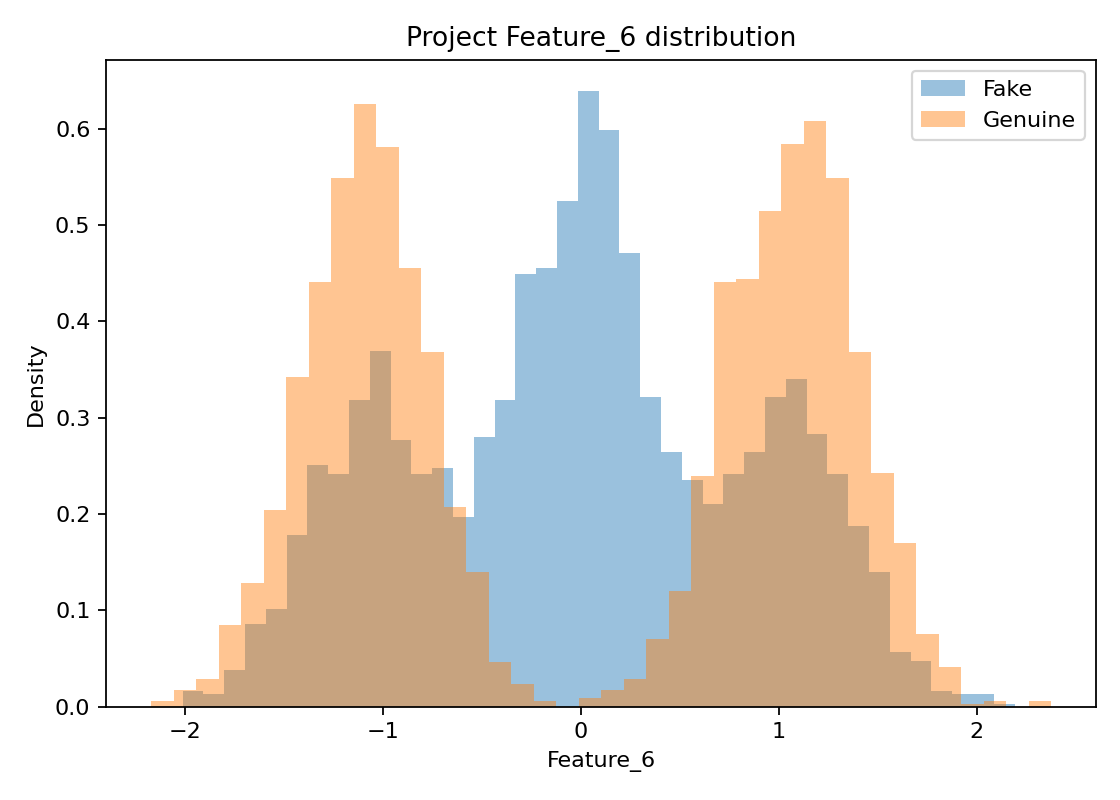
\includegraphics[width=\linewidth]{histograms/feature_6_histogram.png}
        \caption{Histogram of Feature 6, showing Genuine bimodality.}
    \end{minipage}
\end{figure}

\begin{figure}[H]
    \centering
    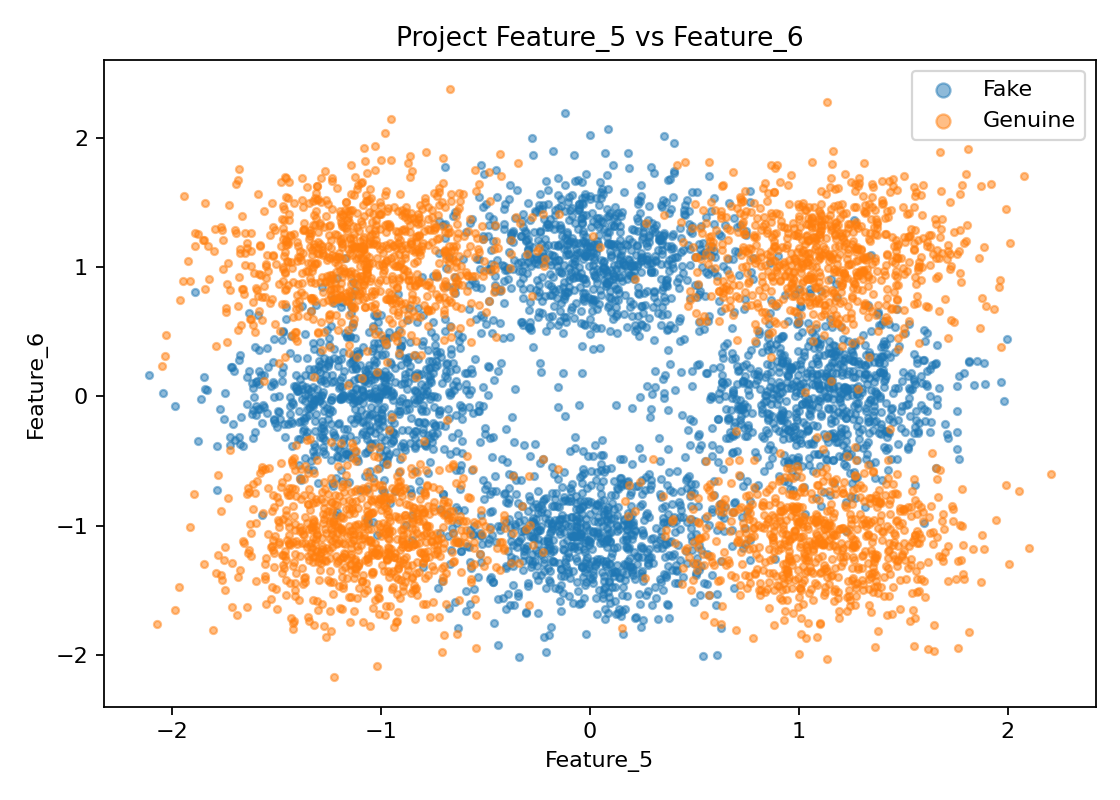
\includegraphics[width=0.6\textwidth]{scatters/features_5_6_scatter.png}
    \caption{Scatter plot of Feature 5 vs Feature 6, illustrating the 4-cluster cross and quadrant topologies.}
    \label{fig:scatter_5_6}
\end{figure}

\subsection*{Theoretical Analysis}

The 2D scatter plot (Figure \ref{fig:scatter_5_6}) resolves the 1D bimodal histograms into explicit, highly structured spatial clusters. Because the Genuine class has distinct peaks at the positive and negative extremes of both axes, it forms a "ring" consisting of exactly \textbf{4 distinct clusters} located in the four diagonal quadrants of the plot (top-left, top-right, bottom-left, bottom-right).

Conversely, the Fake class forms a "cross-like" structure. It also breaks down into roughly \textbf{4 distinct clusters}, but these are located radially along the x and y axes. This creates a geometric grid where the classes interleave perfectly, completely hollowing out the linear separability of the feature space.

\subsection*{Motivation and Future Insights}

The discovery of the 4-cluster topology in Features 5 and 6 is the defining characteristic of this dataset and serves as the mathematical bedrock for our advanced architectural choices in subsequent laboratories:

\begin{enumerate}
    \item \textbf{The Inadequacy of Standard MVG:} A single Multivariate Gaussian distribution (a bell curve) can only model a single center of mass. It cannot physically stretch to cover four isolated quadrants while ignoring the center. Applying a Standard MVG to the Genuine class forces the model to place its mean at $(0,0)$—the exact location of the "valley" where no Genuine data actually exists. This fundamentally compromises the generative log-likelihood estimates.
    \item \textbf{The Necessity of the Gaussian Mixture Model (GMM):} This highly non-Gaussian, multi-cluster topology mathematically necessitates the use of a GMM. By using $M=8$ components (as deployed in our final system), the GMM can assign individual Gaussian spheres to each of the distinct corner clusters, perfectly mapping the true underlying density contours.
    \item \textbf{The Power of the RBF Kernel:} For discriminative models, linear boundaries cannot navigate this grid-like overlap. The Support Vector Machine requires the non-linear projection of the Radial Basis Function (RBF) kernel to draw localized, circular boundaries capable of "wrapping around" the isolated Genuine clusters. This geometrically proves why the GMM and RBF SVM fusion in Laboratory 10 achieved the optimal Minimum DCF.
\end{enumerate}